\documentclass[a4paper]{article}
\usepackage[english]{babel}
\usepackage[utf8]{inputenc}

%
% Graphics
%
\usepackage{graphicx}
\usepackage{xcolor}

\definecolor{alpha}{HTML}{3FA9F5}

%
% Bibliography
%
\usepackage[backend=bibtex,maxnames=5,sorting=none,url=false]{biblatex}
\usepackage{csquotes}

%
% Listings
%
\usepackage{listings}

\definecolor{background}{HTML}{FAFAFA}
\definecolor{sign}{HTML}{3FA9F5}

\lstdefinelanguage{fortune}{
  basicstyle=\ttfamily,
  basewidth={0.5em,0.5em},
  backgroundcolor=\color{background},
  literate=
   *{\%}{{{\color{alpha}{\%}}}}{1}
}

\lstdefinelanguage{shell}{
  basicstyle=\ttfamily,
  basewidth={0.5em,0.5em},
  backgroundcolor=\color{background},
  literate=
    [*]{\\\$}{{{\color{alpha}{\$}}}}{1}
       {Command>}{{{\color{alpha}{Command>}}}}{8}
       {ivan(0)>}{{{\color{alpha}{ivan(0)>}}}}{8}
       {ivan(1)>}{{{\color{alpha}{ivan(1)>}}}}{8}
       {ivan(0):RELEASED>}{{{\color{alpha}{ivan(0):RELEASED>}}}}{17}
       {ivan(0):LOCKED>}{{{\color{alpha}{ivan(0):LOCKED>}}}}{15}
       {ivan(1):LOCKED>}{{{\color{alpha}{ivan(1):LOCKED>}}}}{15}
       {ivan(2):LOCKED>}{{{\color{alpha}{ivan(2):LOCKED>}}}}{15}
}

\lstdefinelanguage{json}{
  basicstyle=\ttfamily,
  basewidth={0.5em,0.5em},
  backgroundcolor=\color{background},
  literate=
   *{:}{{{\color{alpha}{:}}}}{1}
    {,}{{{\color{alpha}{,}}}}{1}
    {\{}{{{\color{alpha}{\{}}}}{1}
    {\}}{{{\color{alpha}{\}}}}}{1}
    {[}{{{\color{alpha}{[}}}}{1}
    {]}{{{\color{alpha}{]}}}}{1}
}

\lstnewenvironment{fortune}%
{\lstset{language=fortune}}%
{}

\lstnewenvironment{json}%
{\lstset{language=json}}%
{}

\lstnewenvironment{shell}%
{\lstset{language=shell}}%
{}

%
% Links
%
\usepackage{hyperref}
\hypersetup{%
  colorlinks=true,
  citecolor={alpha},
  linkcolor={alpha},
  urlcolor ={alpha}
}

%
% Text
%
\newcommand{\ie}{i.e.}
\newcommand{\eg}{e.g.}
\newcommand{\etc}{etc.}

\newcommand{\fix}{should be modified}
\newcommand{\leave}{no changes are needed}
\newcommand{\overwrite}{should contain your previous changes}

\newcommand{\python}{\texttt{Python}}
\newcommand{\classname}[1]{\texttt{#1}}
\newcommand{\filename}[1]{\texttt{#1}}
\newcommand{\code}[1]{\texttt{#1}}

%
% References
%
\newcommand{\sref}[1]{Section~\ref{sec:#1}}
\newcommand{\tref}[1]{Table~\ref{tab:#1}}
\newcommand{\fref}[1]{Figure~\ref{fig:#1}}

\newcommand{\slabel}[1]{\label{sec:#1}}
\newcommand{\tlabel}[1]{\label{tab:#1}}
\newcommand{\flabel}[1]{\label{fig:#1}}

\newcommand{\slab}[1]{\label{sec:#1}}
\newcommand{\tlab}[1]{\label{tab:#1}}
\newcommand{\flab}[1]{\label{fig:#1}}

\newcommand{\aref}[1]{Lab~#1 \cite{description#1}}


\bibliography{include/references.bib}

\title{Distributed Systems: Lab 3\\Middleware: Peer-to-Peer
Communications}
\author{Petru Eles and Ivan Ukhov\\
\vspace{0.5em}
\href{mailto:petru.eles@liu.se}{petru.eles@liu.se} and \href{mailto:ivan.ukhov@liu.se}{ivan.ukhov@liu.se}
}
\date{January 24, 2016}

\begin{document}
\maketitle

\section{Introduction}
\begin{figure}
  \centering
  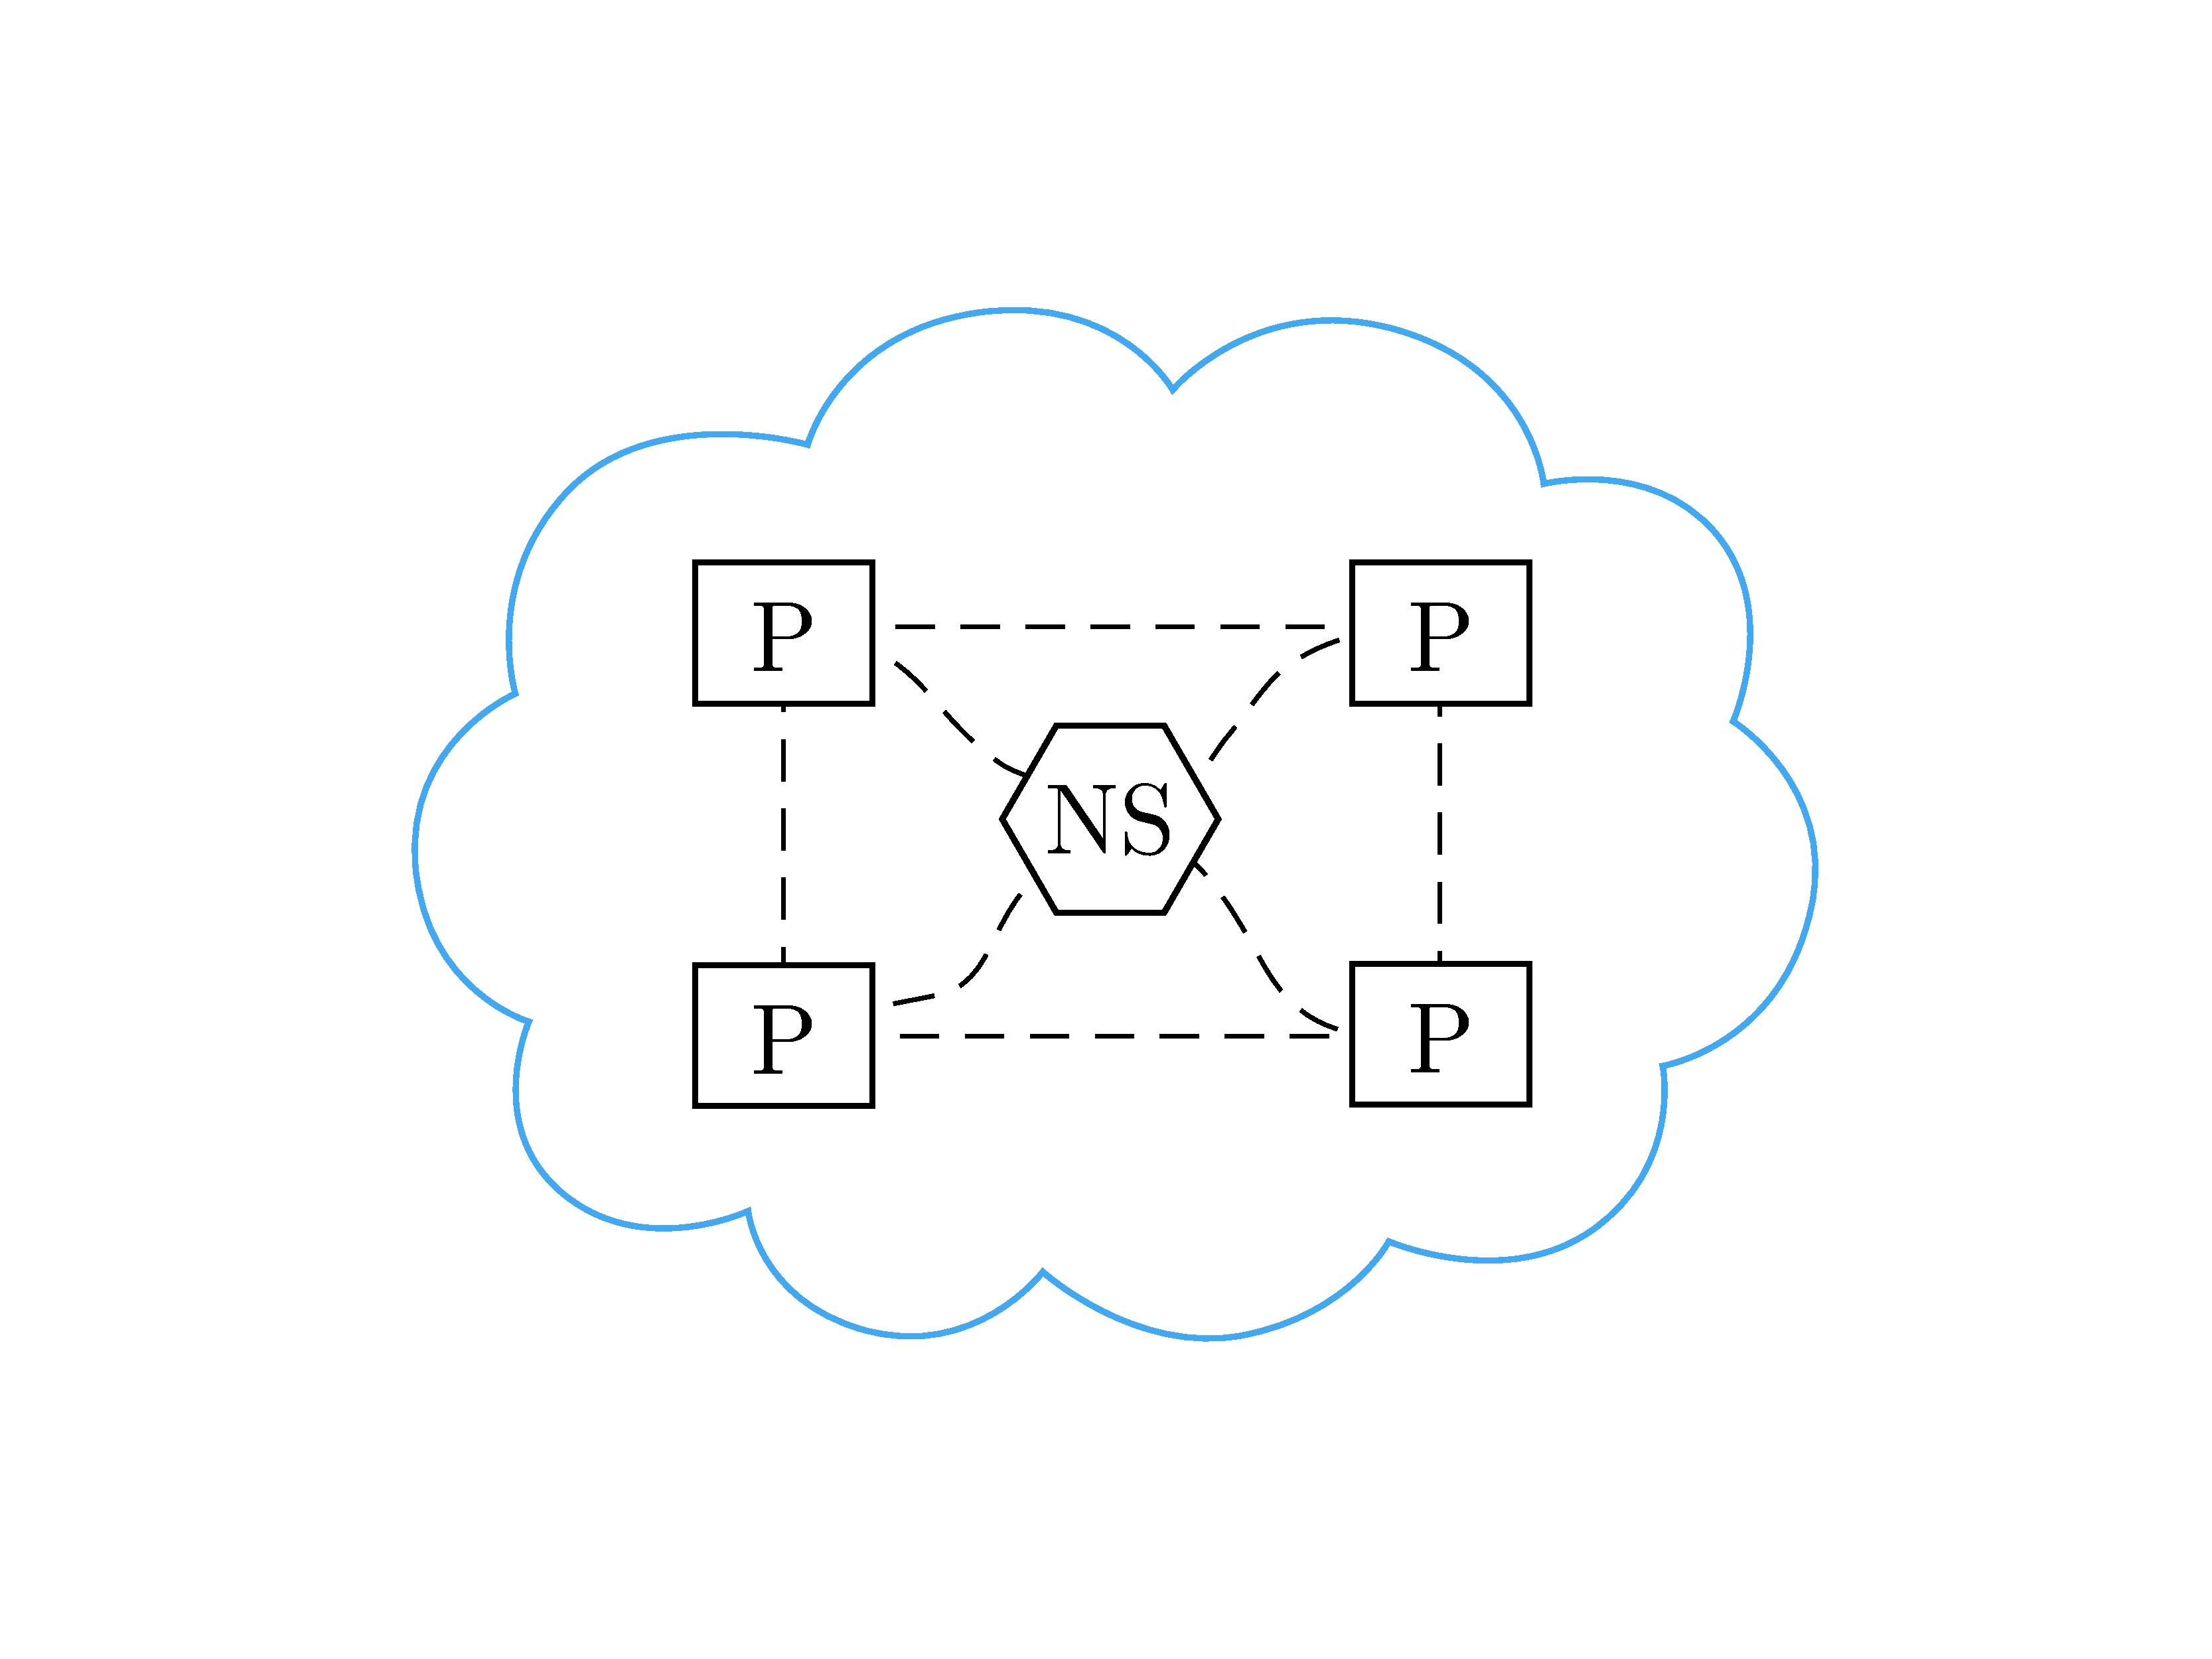
\includegraphics[width=0.8\textwidth, clip=true, trim=0 180px 0 180px]{include/assets/chat.pdf}
  \caption{A name service (NS) and a number of chat-peers (P). First, the peers discover each other by means of the name service, and then they start exchanging messages directly.}
  \flabel{chat}
\end{figure}

The goal of the current lab is to make the code written for \aref{2} properly
handle situations when peers arbitrary join and leave your distributed system.
This functionality will be delegated to a separate class called
\classname{PeerList}, which will take advantage of the object request broker
implemented as a part of the previous lab. In addition, you will introduce
interactions between peers themselves, \ie, peers will be remotely invoking
methods \cite{lecture3} of each other (as you remember, so far peers were
communicating only with the name service). In order to put all these pieces
together and ensure that they work properly, you will implement a test
application for exchanging text messages between peers. Such a system of
messengers is depicted in \fref{chat}.

\section{Your Task}
\subsection{Preparation}
Continue working with the same code base that you have been working with so far,
including all the changes that you have made. The files relevant to this lab are
listed below. You should read and understand them.
\begin{itemize}

  \item \filename{lab3/chatPeer.py} --- the chat application (\leave);

  \item \filename{lab3/test.sh} --- a shell script that you can use for testing;

  \item \filename{modules/Common/nameServiceLocation.py} --- the same as for
  \aref{2} (\leave);

  \item \filename{modules/Common/objectType.py} --- the same as for \aref{2}
  (\overwrite);

  \item \filename{modules/Common/orb.py} --- the same as for \aref{2}
  (\overwrite);

  \item \filename{modules/Common/wrap.sh} --- the same as for \aref{1};

  \item \filename{modules/Server/peerList.py} --- the module that maintains a
  list of peers of a given object type (\fix).

\end{itemize}

The main functionality of this lab is concentrated in \filename{peerList.py},
which contains the \classname{PeerList} class. As the name suggests, this class
represents a list of peers, and it is utilized as follows. Each peer has an
instance of \classname{PeerList}, and this instance maintains local images, that
is, \classname{Stub}s, of all the peers that are currently present in the
network (restricted to your name space specified by your object
type\footnote{Object types were discussed in \aref{2}.}). Therefore, whenever a
peer wants to invoke a method of some other peer, it just needs to find the
addressee in the peer list and make a call to the corresponding image; the rest
will be done automatically by the object-request-broker functionality that you
implemented earlier. Carefully read the code in \filename{peerList.py} and
understand what it does. In particular, ensure that you understand the purpose
of the locks utilized throughout the module.

Run \filename{chatPeer.py} in several terminal windows. If you have overwritten
\filename{orb.py} with your correct implementation from \aref{2}, the
application should start without any errors and display its menu as shown
below:\footnote{As you have probably discovered in the code, you can specify
your object type with the \texttt{-t} command argument instead of editing
\filename{objectType.py}.}
\begin{shell}
\$ ./chatPeer.py -t ivan
Choose one of the following commands:
    l                       ::  display the peer list,
    <PEER_ID> : <MESSAGE>   ::  send <MESSAGE> to <PEER_ID>,
    h                       ::  print this menu,
    q                       ::  exit.
ivan(1)> l
List of peers of type `ivan':
ivan(1)> 2 : Can anybody hear me?
Cannot send messages to 2. Make sure it is in the list of peers.
ivan(1)>
\end{shell}
Unfortunately, this instance of the application cannot see the other instances,
which are running in parallel, and, therefore, cannot send messages to them.

\subsection{Implementation}
The \classname{PeerList} class has two missing parts, which you are asked to
implement. More specifically, the two parts are in the \code{initialize} and
\code{destroy} functions, and you should complete them as follows:
\begin{itemize}

  \item \code{initialize} --- the function populates the peer list of a newly
  started peer and notifies the other peers about this event. To this end, the
  function should (a) request the peer list of your name space from the name
  service and (b) register the current peer in each peer from the obtained list.

  \item \code{destroy} --- the function is called whenever the peer that owns
  this instance of \classname{PeerList} leaves the system. The function should
  unregister the peer by calling an appropriate method of each peer in the peer
  list.

\end{itemize}
As usual, there is the following requirement to your implementation:
\begin{itemize}

  \item Your peers should be resistant to potential exceptions that can happen
  during remote method invocation; ensure that your peers stay alive.

\end{itemize}
After the implementation has been completed, run the system once again and make
sure that now you can exchange messages without any problems. Use the test
script to start several clients at once.

\section{Conclusion}
At this point, you have a rather solid ground for your future distributed
database of fortunes. Now you can perform remote method invocations in a
straightforward manner, thanks to your object request broker and peer list.
However, we shall postpone the integration of this code with the
database-related code from \aref{1} until the final lab. The reason is that
there is one crucial component which is still missing. This component is a
distributed lock \cite{lecture67}, which you will closely look at in \aref{4}.

\printbibliography

\end{document}
